\section{Results}

\subsection{Comparison of Fit vs Non-Fit}

\begin{figure}
    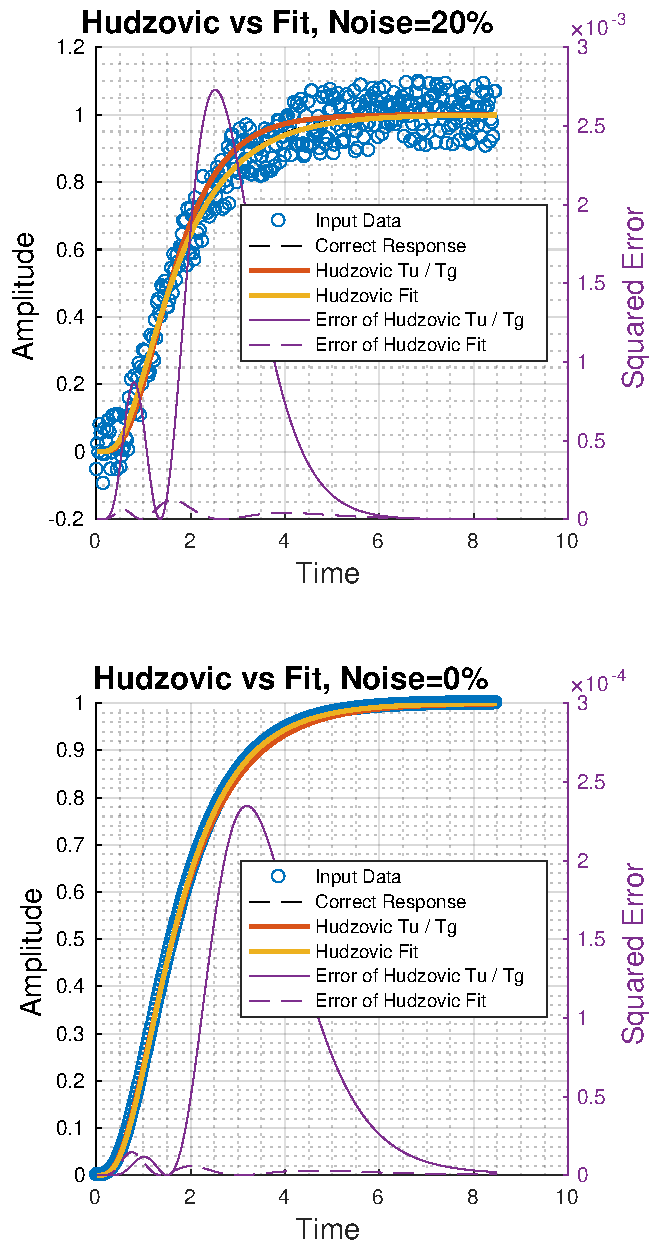
\includegraphics[width=\linewidth]{images/hudzovic_vs_fit}
    \caption{Comparison of a normal Hudzovic Tu/Tg lookup to a least square refinement. Order n=4, Noise=20\% and 0\%}
    \label{fig:hudzovic_vs_fit}
\end{figure}

\begin{figure}
    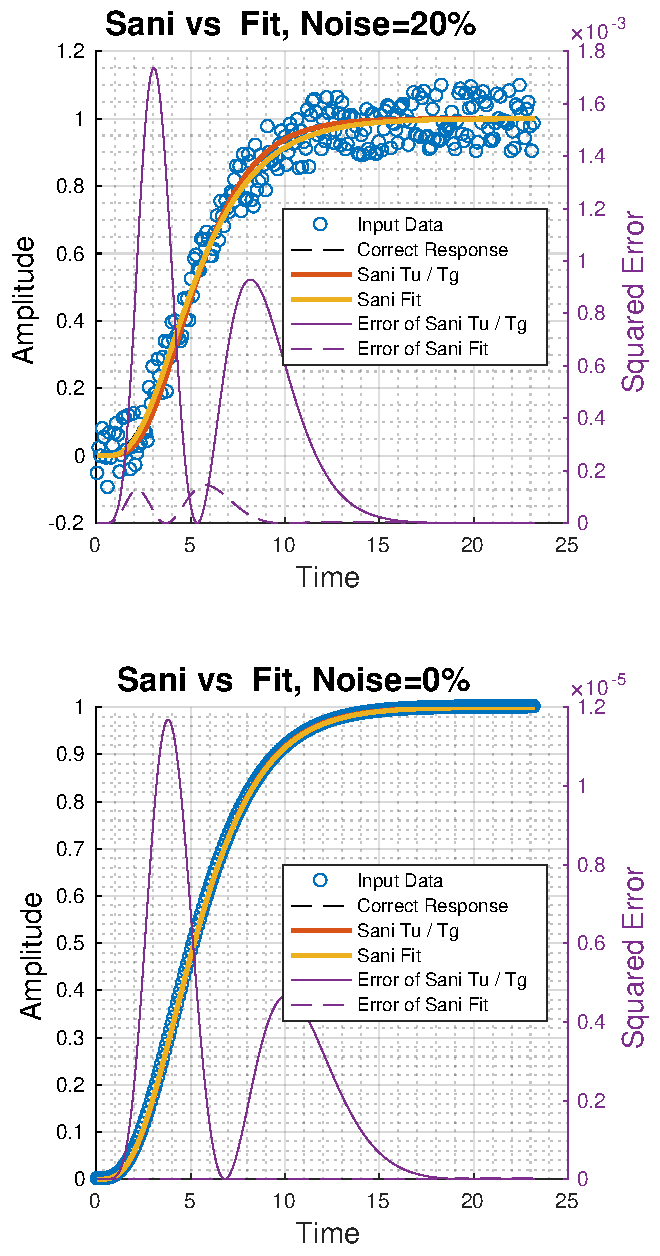
\includegraphics[width=\linewidth]{images/sani_vs_fit}
    \caption{Comparison of a normal Sani Tu/Tg lookup to a least square refinement. Order n=4, Noise=20\% and 0\%}
    \label{fig:sani_vs_fit}
\end{figure}


\subsection{Comparison of Accuracy}

The big question is: What is the best method?

To answer this question, a  total  amount  of  1000  simulations were performed,
where the noise amplitude  on  the  input step response function was increased a
bit after each iteration. The input step response  function  was  a PT4 element,
constructed  by using Hudzovic's method with $r=0.5$,  $n=4$,  and  $T=1$.  This
particular function was chosen because it yielded the  most  stable  results  in
previous tests.

The ever  increasing  noisy  input  function  was fed into each of the 6 methods
outlined in this report. Each method's result was then compared to the original,
non-noisy input function by calculating the mean squared error.

The resulting error data was fed through a sliding average filter of  width  10,
resulting in figure \ref{fig:error_noise}.

\begin{figure}
    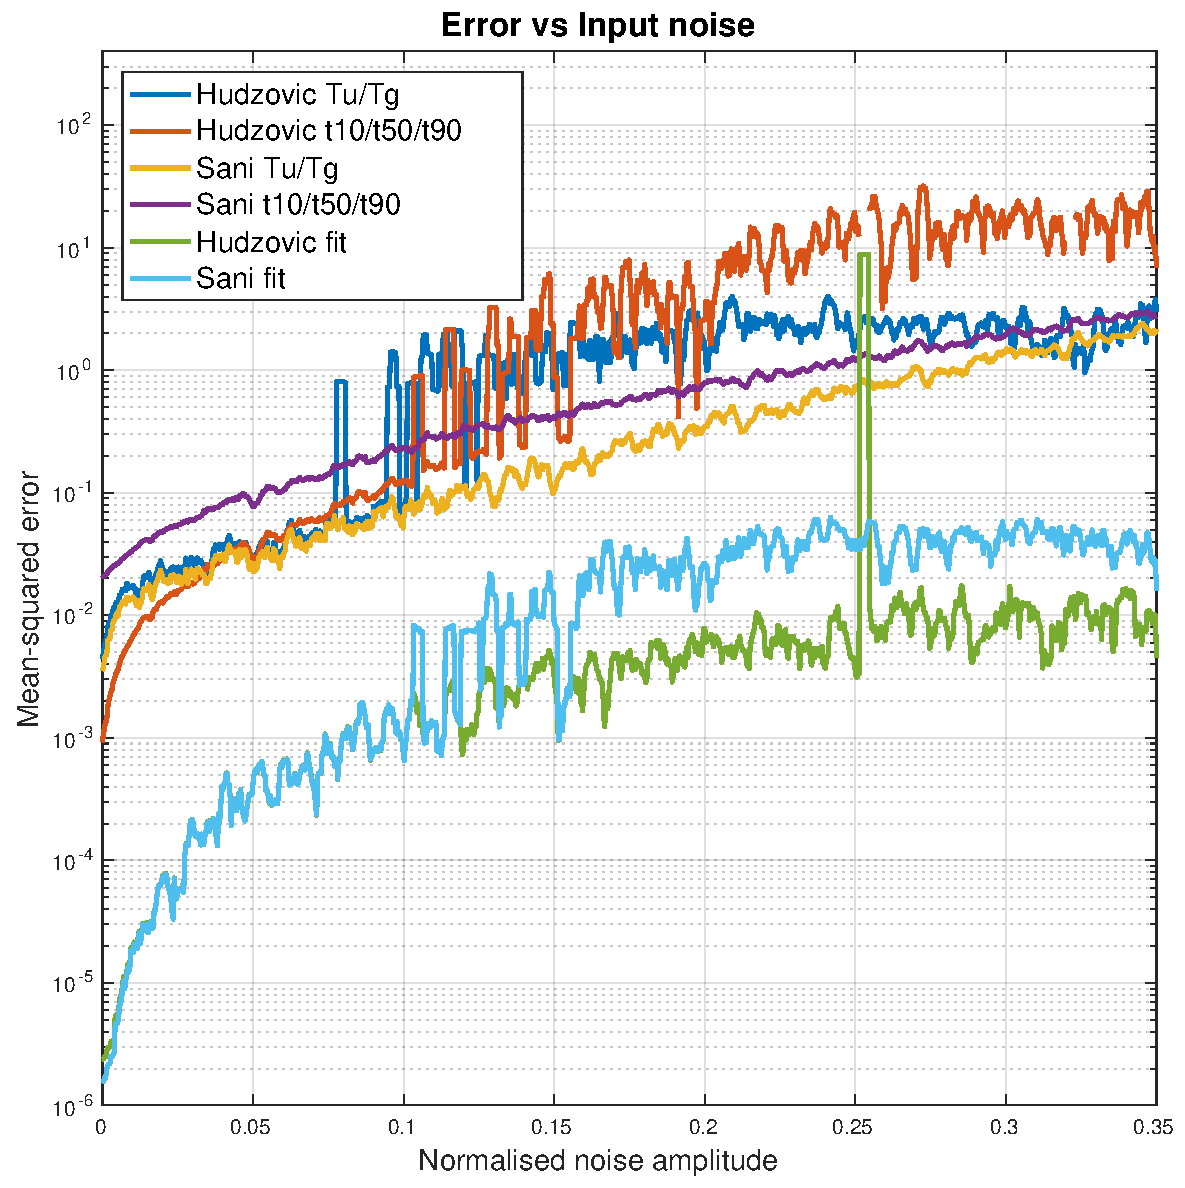
\includegraphics[width=\linewidth]{images/error_noise}
    \caption{The root mean square error (RMSE) of each method to the original step response function, in function of normalised input noise amplitude.}
    \label{fig:error_noise}
\end{figure}

\begin{figure}
    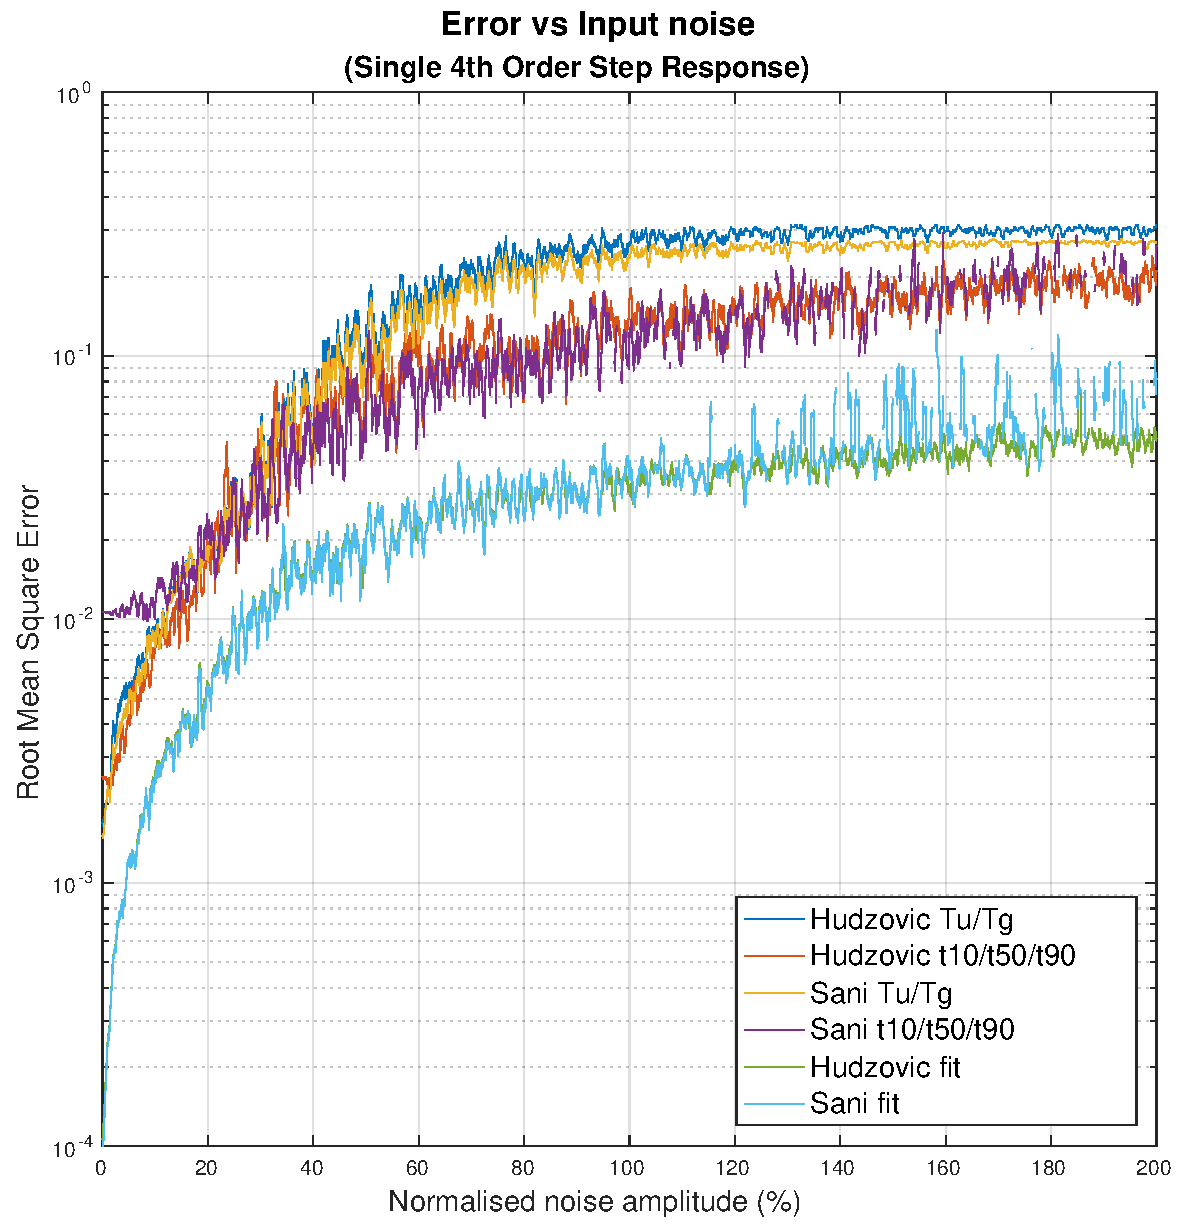
\includegraphics[width=\linewidth]{images/error_noise_long_term}
    \caption{Long term view of the root mean square error (RMSE) of each method to the original step response function, in function of normalised input noise amplitude.}
    \label{fig:error_noise_long_term}
\end{figure}

An  immediate  conclusion  to be drawn is that the two fitting methods (cyan and
olive curves) yield more accurate results than any  of  the  other methods by an
order of magnitude. This is to be expected, of course. While the Sani fit proves
itself to be  the  most accurate fitting method for non-noisy signals, as can be
seen by zooming into the bottom left of the plot, the Hudzovic fit proves itself
to be the most accurate for very noisy signals.

The exact reason as to why this happens is due  to  the nature of how Hudzovic's
method works. In Hudzovic's  approach,  equation  \ref{eq:hudzovic},  if  $n$ is
chosen higher or lower  than  the  correct order (which can happen randomly with
noisy input signals), the resulting ``misshaped'' curve doesn't deviate from the
correctly  shaped curve \textit{as  much}  as  Sani's  approach  using  equation
\ref{eq:sani}. \todo{visualise this with a plot or something} \todo{Is this even
true?}

A (personally) unexpected  result  is  that Hudzovic's characterisation approach
with  $T_u/T_g$  shows  to  be  more  accurate for  noisy  signals  than  Sani's
characterisation  approach  using $t_{10}$,  $t_{50}$,  $t_{90}$.  This  can  be
observed  by comparing the (orange) and  (blue)  curves,  or  by  comparing  the
(purple) and (yellow) curves. This result is unexpected because of how $T_u/T_g$
is calculated: The derivative of  the  signal  must be computed in order to find
the point of inflection (see theory section). The  derivative  of a noisy signal
is, of course, an even noisier signal, \todo{show this with a plot or something}
which should make correctly  calculating  the  point  of  inflection  much  less
accurate  than calculating the threshold values  $t_{10}$,  $t_{50}$,  $t_{90}$.

Interestingly, the  most accurate non-fitting method is Hudzovic's approach, but
by using $t_{10}$, $t_{50}$, $t_{90}$ instead of  $T_u/T_g$.  This  is only true
for cleaner input signals with a normalised noise amplitude of less  than  0.05.
To get a feeling  for  what that means, see figure \todo{create figure with 0.05
normalised noise}

After that, for noisier signals,  the most accurate non-fitting method is Sani's
approach   paired   with   Hudzovic's   $T_u/T_g$   characterisation   approach.


\subsection{Comparison of Accuracy vs Order}

Another  interesting  question  is:  Does  the accuracy change depending on  the
transfer function's order $n$?

For each order ($n=[2..8]$) 100 randomly generated  PTn  transfer functions were
generated and their step response was fed into each  method.  The step responses
from each method's transfer function were then  compared with the original input
function's step response and the root mean square error (RMSE)  was  calculated.
The  100  errors  were then averaged, resulting in a final error value for  each
method, for each order.

\begin{figure}
    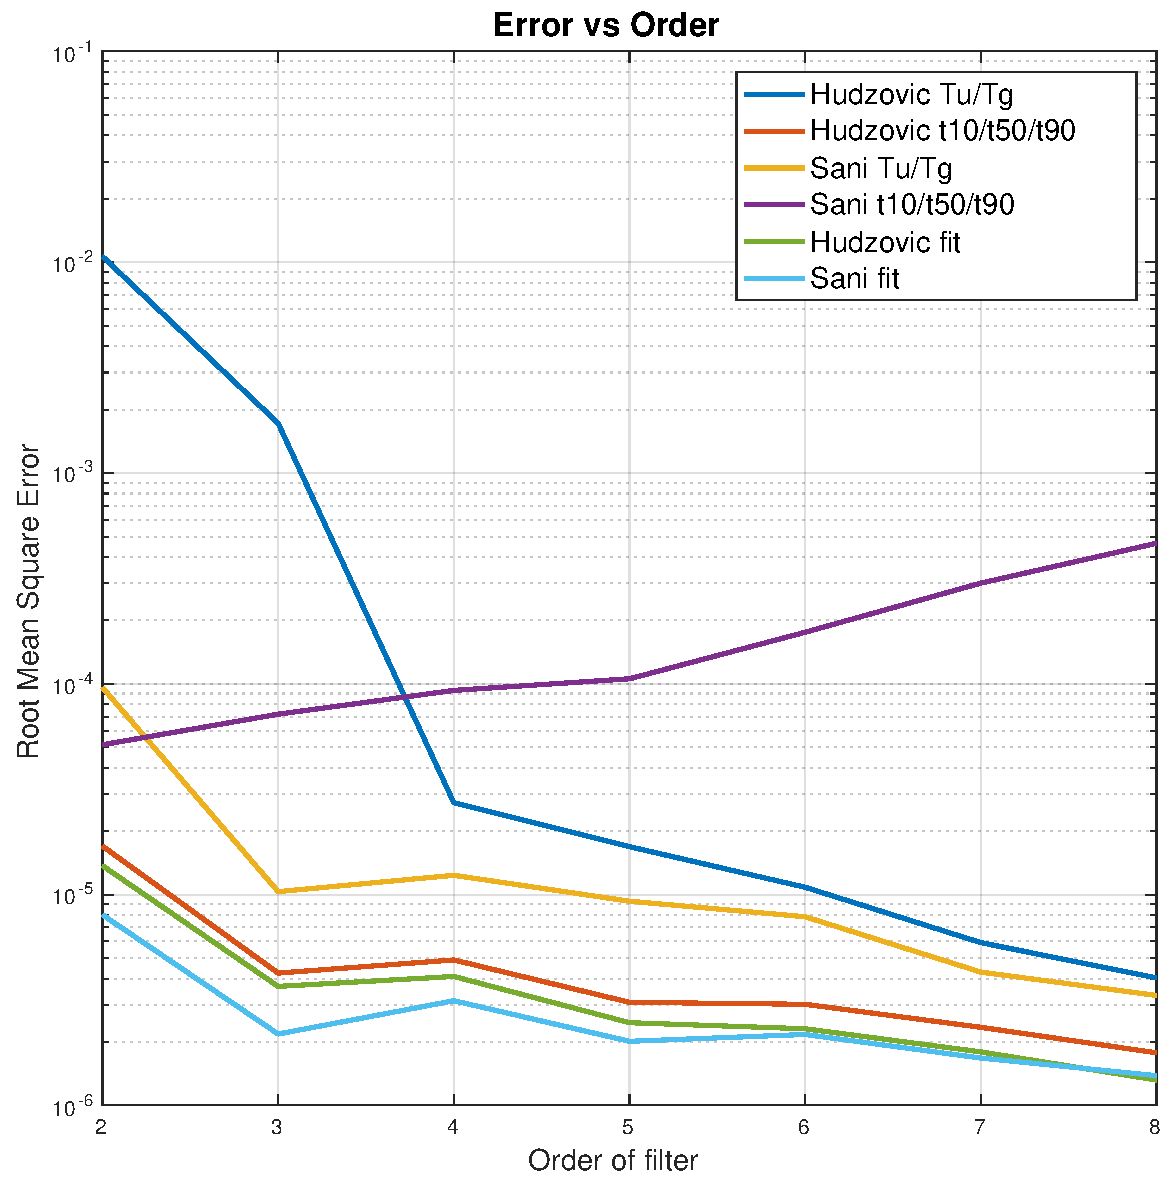
\includegraphics[width=\linewidth]{images/error_order}
    \caption{The mean square error (MSE) of each method to a randomly generated step response, in function of filter order}
    \label{fig:error_order}
\end{figure}

The data portrayed in figure \ref{fig:error_order} shows these errors.

A first observation to make is that the  resulting  data  points  for  4th order
transfer  functions correlate with the data seen in figure \ref{fig:error_noise}
for when the noise is low  or  non-existent,  gives  gives the validity of these
results some confidence.

As expected, the fitted methods  yielded the most accurate results. The Sani fit
proves  to be better than the Hudzovic fit.

An interesting observation is that the method proposed by L. Sani\cite{ref:sani}
using the $t_{10}$, $t_{50}$, $t_{90}$ characterisation performs worse and worse
the  higher  the order, whereas all other methods perform better and better. The
exact reason as to why this happens is related  to  the interpolation formulae proposed by L. Sani  \todo{reference  to
theory section}.

\begin{figure}
    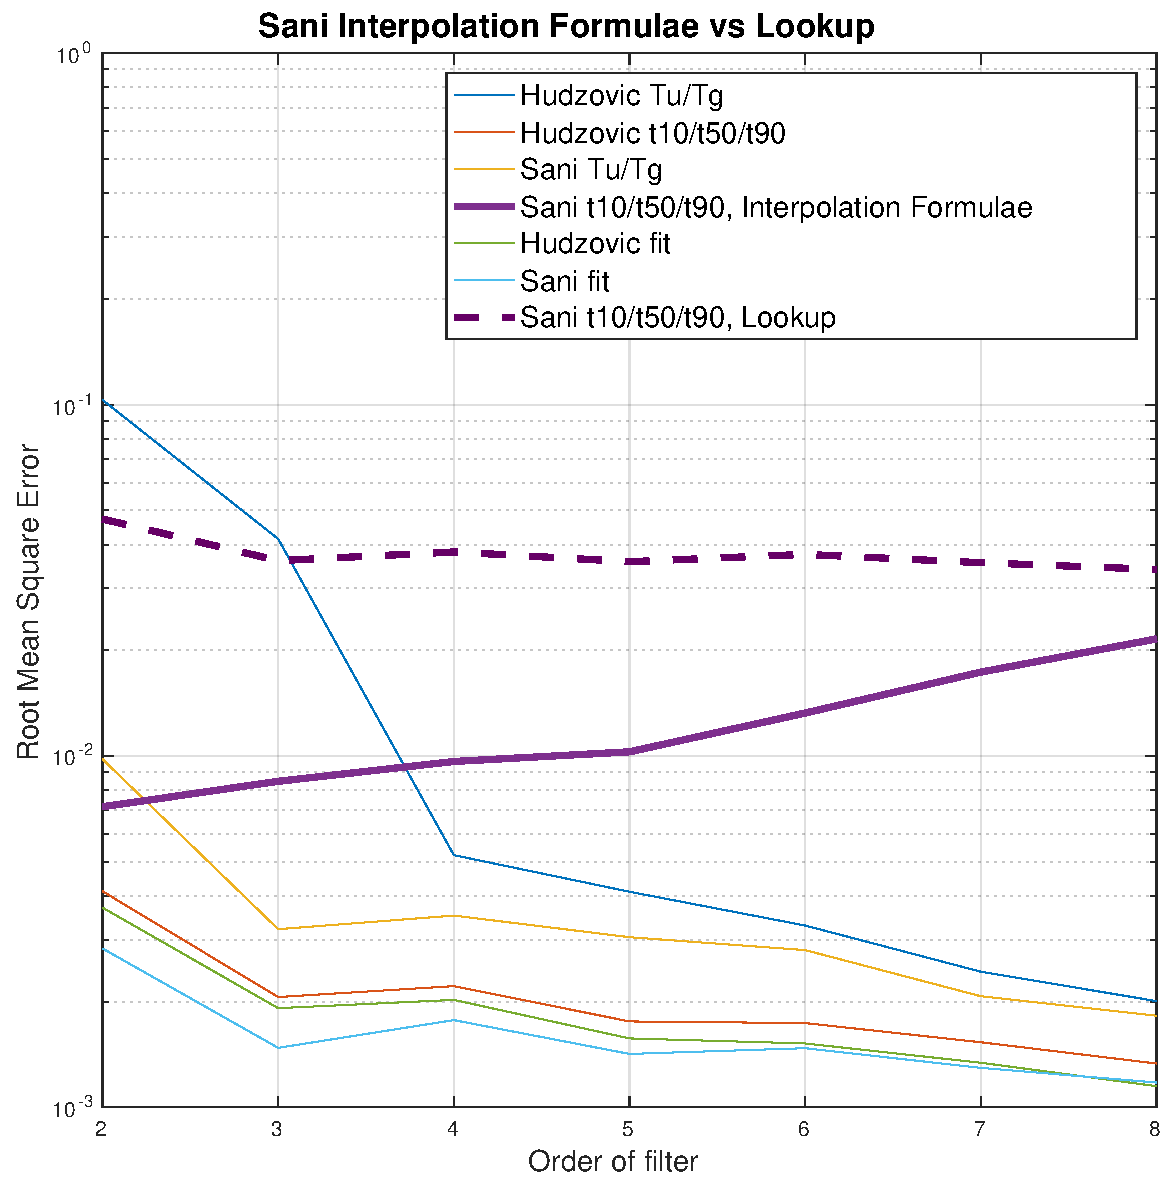
\includegraphics[width=\linewidth]{images/sani_interpolation_vs_lookup}
    \caption{Interpolation formulae proposed by L. Sani compared to ``brute force'' calculating the individual t10, t50, t90 parameters and creating lookup curves}
    \label{fig:interpolation_vs_lookup}
\end{figure}

\todo{Worth investigating a more accurate method of determining t10, t50, t90}

